\documentclass[tikz, border=1mm]{standalone}
\usepackage{tikz} 
\usetikzlibrary{arrows.meta}
\usepackage{pgfplots}

\begin{document}

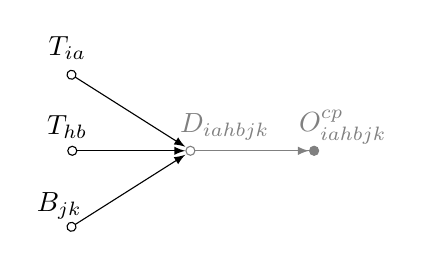
\begin{tikzpicture}

    % outcome
    \node[gray] at (3.5,1) {$O^{cp}_{iahbjk}$}; %[gray]

    % difference
    \node[gray] at (2,1) {$D_{iahbjk}$}; %[gray]
    \draw[{Circle[open]}-{latex}{Circle},gray](1.5,0.7) to (3.2,0.7); %,gray

    %%%%%%%%%%%%%%%%%%%%%%%%%%%%%%%%%%%%%%%%%%%%%%%%%%%%%%%%%

    % "true" discriminal process for sub-unit
    \node at (0,2) {$T_{ia}$}; %[gray]
    \draw[{Circle[open]}-{latex}](0,1.7) to (1.5,0.75); %,gray 
    
    % "true" discriminal process for sub-unit
    \node at (0,1) {$T_{hb}$}; %[gray]
    \draw[{Circle[open]}-{latex}](0,0.7) to (1.5,0.7); %,gray
    
    % judges' biases
    \node at (-0.1,0) {$B_{jk}$}; %[gray]
    \draw[{Circle[open]}-{latex}](0,-0.3) to (1.5,0.65); %,gray     
    
\end{tikzpicture}

\end{document}
